\documentclass{article}
\usepackage{helvet}


\usepackage{cite}
\usepackage{amsmath,amssymb,amsfonts}
\usepackage{algorithmic}
\usepackage{graphicx}
\usepackage{textcomp}
\usepackage{xcolor}
\usepackage{hyperref}
\usepackage{placeins}
\usepackage{graphicx}
\usepackage{subcaption}



\def\BibTeX{{\rm B\kern-.05em{\sc i\kern-.025em b}\kern-.08em
    T\kern-.1667em\lower.7ex\hbox{E}\kern-.125emX}}


\title{Question 4, Assignment 3: CS 754, Spring 2024-25}
\author{
\IEEEauthorblockN{
    \begin{tabular}{cccc}
        \begin{minipage}[t]{0.23\textwidth}
            \centering
            Amitesh Shekhar\\
            IIT Bombay\\
            22b0014@iitb.ac.in
        \end{minipage} & 
        \begin{minipage}[t]{0.23\textwidth}
            \centering
            Anupam Rawat\\
            IIT Bombay\\
            22b3982@iitb.ac.in
        \end{minipage} & 
        \begin{minipage}[t]{0.23\textwidth}
            \centering
            Toshan Achintya Golla\\
            IIT Bombay\\
            22b2234@iitb.ac.in
        \end{minipage} \\
        \\ 
    \end{tabular}
}
}

\date{March 21, 2025}


\usepackage{amsmath}
\usepackage{amssymb}
\usepackage{hyperref}
\usepackage{ulem,graphicx}
\usepackage[margin=0.5in]{geometry}

\begin{document}
\maketitle

\textbf{Declaration:} The work submitted is our own, and
we have adhered to the principles of academic honesty while completing and submitting this work. We have not
referred to any unauthorized sources, and we have not used generative AI tools for the work submitted here.

\begin{enumerate}
\item Consider the image `cryoem.png' in the homework folder. It is a 2D slice of a 3D macromolecule in the well-known EMDB database. Generate $N$ Radon projections of this 2D image at angles drawn uniformly at random from $0$ to $360$ degrees. Your job is to implement the Laplacian eigenmaps based algorithm for 2D tomographic reconstruction from unknown angles, given these projection vectors. You should test your algorithm for $N \in \{50,100,500,1000,2000,5000,10000\}$. In each case, display the reconstructed image, and compute its RMSE appropriately normalized for rotation. (Note that cryo-EM reconstructions are valid only up to a global rotation, so direct RMSE computation without compensating for the arbitrary rotation is meaningless). You can use the routines \texttt{radon}, \texttt{imrotate} in MATLAB. \textsf{[30 points]}
\\
    \makebox[0pt][l]{\hspace{-7pt}\textit{Soln:}} % Aligns "Answer:" to the left
\\
The reconstructed images along with their corresponding RMSE values are as follows:
\FloatBarrier
\begin{figure}[!h]
    \centering
    \begin{tabular}{cc}
        % Row 1
        \begin{subfigure}{0.45\textwidth}
            \centering
            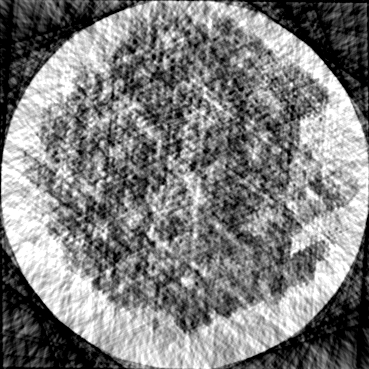
\includegraphics[width=0.65\linewidth]{HomeWork_3/3/images/reconstructed_N_50.png}
            \caption{N = 50, RMSE = 0.1593}
        \end{subfigure} &
        \begin{subfigure}{0.45\textwidth}
            \centering
            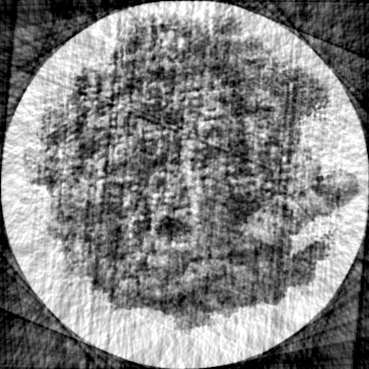
\includegraphics[width=0.65\linewidth]{HomeWork_3/3/images/reconstructed_N_100.png}
            \caption{N = 100, RMSE = 0.1203}
        \end{subfigure} \\
        
        % Row 2
        \begin{subfigure}{0.45\textwidth}
            \centering
            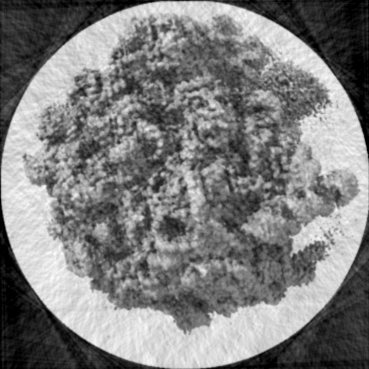
\includegraphics[width=0.65\linewidth]{HomeWork_3/3/images/reconstructed_N_500.png}
            \caption{N = 500, RMSE = 0.0584}
        \end{subfigure} &
        \begin{subfigure}{0.45\textwidth}
            \centering
            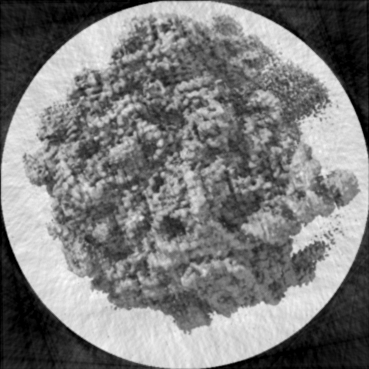
\includegraphics[width=0.65\linewidth]{HomeWork_3/3/images/reconstructed_N_1000.png}
            \caption{N = 1000, RMSE = 0.0502}
        \end{subfigure} \\
    \end{tabular}
\end{figure}

\clearpage  % Forces the next set of images onto a new page

\FloatBarrier
\begin{figure}[!h]
    \centering
    \begin{tabular}{cc}
        % Row 3
        \begin{subfigure}{0.45\textwidth}
            \centering
            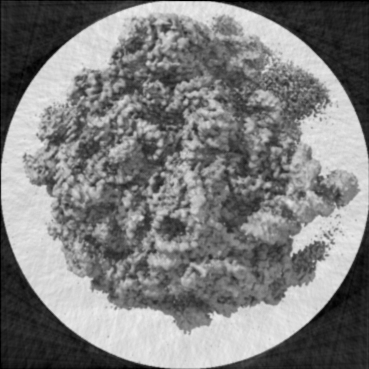
\includegraphics[width=0.65\linewidth]{HomeWork_3/3/images/reconstructed_N_2000.png}
            \caption{N = 2000, RMSE = 0.0359}
        \end{subfigure} &
        \begin{subfigure}{0.45\textwidth}
            \centering
            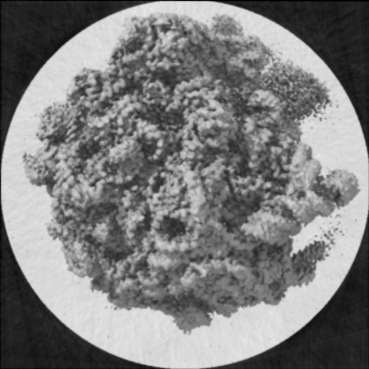
\includegraphics[width=0.65\linewidth]{HomeWork_3/3/images/reconstructed_N_5000.png}
            \caption{N = 5000, RMSE = 0.0279}
        \end{subfigure} \\
        
        % Row 4
        \begin{subfigure}{0.45\textwidth}
            \centering
            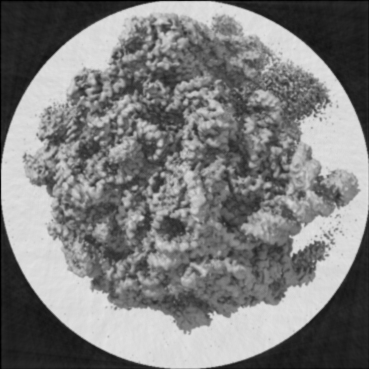
\includegraphics[width=0.65\linewidth]{HomeWork_3/3/images/reconstructed_N_10000.png}
            \caption{N = 10000, RMSE = 0.0262}
        \end{subfigure} &
        \begin{subfigure}{0.45\textwidth}
            \centering
            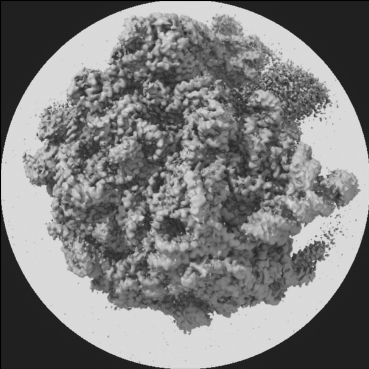
\includegraphics[width=0.65\linewidth]{HomeWork_3/3/images/cryoem.png}
            \caption{Original Image}
        \end{subfigure} \\
    \end{tabular}
\end{figure}
\end{enumerate}
\end{document}